\documentclass[a4paper]{scrartcl}
\usepackage[utf8]{inputenc}
\usepackage[english]{babel}
\usepackage{graphicx}
\usepackage{lastpage}
\usepackage{pgf}
\usepackage{wrapfig}
\usepackage{fancyvrb}
\usepackage{fancyhdr}
\usepackage{hyperref}
\pagestyle{fancy}

\catcode`\_=\active
\protected\def_#1_{\textit{#1}}

% Create header and footer
\headheight 27pt
\pagestyle{fancyplain}
\lhead{\footnotesize{Network Programming, ID1212}}
\chead{\footnotesize{Web services}}
\rhead{}
\lfoot{}
\cfoot{\thepage}
\rfoot{}

% Create title page
\title{Assignment 4 - Web services}
\subtitle{Network Programming, ID1212}
\author{Bernardo Gonzalez Riede, begr@kth.se}
\date{\today}

\begin{document}

\maketitle

%Introduction
\section{Introduction}
Goals:
\begin{itemize}
	\item Develop a three-tier web-based application using frameworks
	\item Deploy and run a web-based application on an application server.
\end{itemize}


%Literature
\section{Literature Study}
As in previous assignments, the main source were the video lectures on the topic and the example code.

%Literature
\section{Method}
As in previous assignments, the mvc approach has been used again to layer the program.

The choice for a database fell on MySQL because of past works with it.
The implementation was realized in Netbeans in Java 8 EE using Pyara as the application server.


\section{Result}

Link to public Github repository with code:
\href{https://github.com/MemBernd/ID1212-Web-services}{https://github.com/MemBernd/ID1212-Web-services}

\subsection{Layering}
The layering of the application is divided into four layers:
\begin{itemize}
	\item The _view_ holds the JSF page.
	\item The _controller_ holds a ``normal'' java class.
	\item The _model_ holds the JPA entities.
	\item The _storage_ holds the EJB, a class responsible for connecting to the MySQL database.
\end{itemize}


%subsection covering persistent storage stuff
\subsection{Database}
The database in \ref{fig:database} consists of two tables.
The first table acts as a catalog, holding the different currencies, while the second one is the result of a many to many association of the catalog to itself.

\begin{figure}[h!]
  \begin{center}
    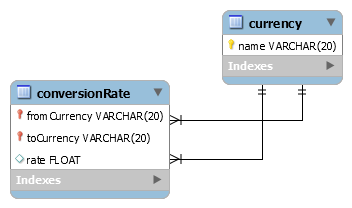
\includegraphics[scale=0.8]{db.png}
    \caption{Table relations in database.}
    \label{fig:database}
  \end{center}
\end{figure}



%subsection covering rmi stuff
\subsection{Frameworks}

\subsubsection{JSF}


\subsubsection{EJB}



\subsubsection{JPA}



\subsection{Client side}
The user can access the application through a browser, which presents him with the jsf (see \ref{fig:ui}).
The user is able to select between 4 currencies to convert between them.
In case he selects the same currency, the application will return, hence show, the same amount as entered.

\begin{figure}[h!]
  \begin{center}
    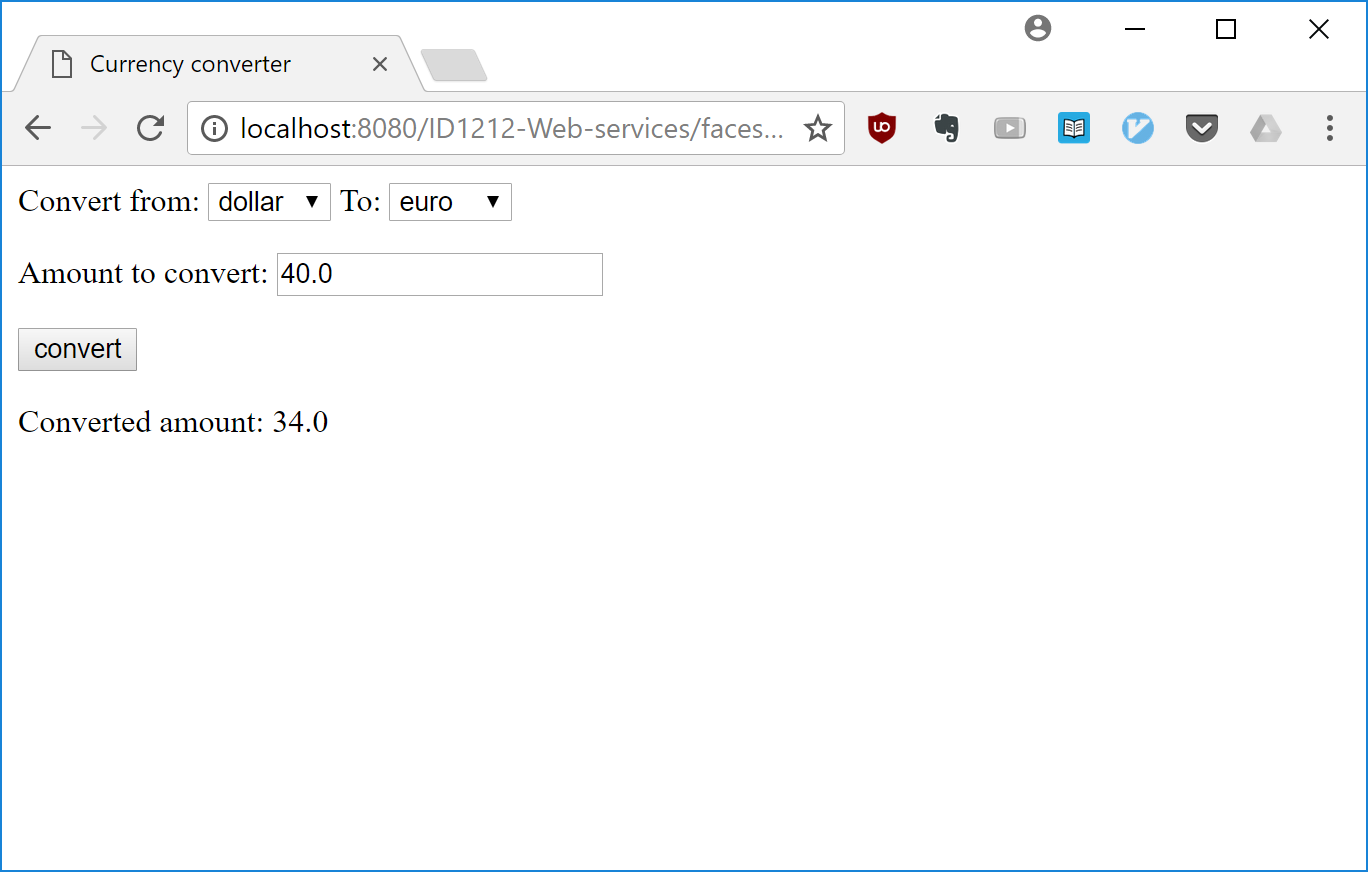
\includegraphics[scale=0.5]{ui.png}
    \caption{Browser interface}
    \label{fig:ui}
  \end{center}
\end{figure}

%subsection discussion
\section{Discussion}
Through the use of comboboxes the incorrect input is limited to the use of non digits in the currency amount.
Through the use of Beans, this behaviour is captured instantly and the user is shown a messaeg similar to:
\\_ 'XX' must be a number consisting of one or more digits._

%subsection comments
\section{Comments About the Course}

It tool around
\begin{itemize}
        \item  for coding.
        \item for the report.
        \item  watching videos, taking notes and thinking about how to tackle the problem.
\end{itemize}




\end{document}
